\documentclass[11]{article}

\usepackage[backend=bibtex]{biblatex}
\bibliography{export}

\usepackage{amsmath}
\usepackage[inline]{enumitem}
\usepackage{graphicx}
\usepackage{gensymb}
\usepackage{float}
\newcommand{\dd}[1]{\mathrm{d}#1}
\usepackage{hyperref} 

\usepackage[T1]{fontenc}
\usepackage[utf8]{inputenc}
\usepackage[font=small,labelfont=bf]{caption}

\usepackage[dvipsnames]{xcolor}

\usepackage{bm}

\author{}

\title{Optimal Gaze Control Through Reinforcement Learning}

\begin{document}
\maketitle 	

\section{Introduction}
Humans achieve near optimal performance in visual perception tasks\cite{najemnik2005,knill2004} despite employing a mostly noisy sensory information.
For example, photon sensitive cells fire seemingly randomly at incoming stimuli as activity in low light is accompanied by continuous noise\cite{baylor1984,vanrossum1998,field2002}.  
More so, the ocular globe has a non-uniform distribution of sensory cells.
Whilst the majority of cells are located in a central area called the fovea, the peripheral regions are coarse\cite{jonas1992,purves2001}. 
The difference in cell density and size leads to a clear perception at the center of vision and imprecise perception for peripheral view.  
In spite of such noisy and imprecise apparatus, humans are able to act near optimally to the surrounding environment. 

It is believed that the brain adopts methods of Bayesian inference to reduce sensory uncertainty and deduce the true state of the world\cite{rao2010,knill2004}.
As new visual information is collected, internal representations about the world become more precise and certain.
However, if multiple activities compete over sensory input, one must prioritise information gathering.
That is, optimal behaviour would elucidate the state of the world selectively, in favour of the task having highest importance.

We posit that gaze behaviour requires a combination of reward and level of uncertainty to determine the optimal place of focus.
The process has importance to the field of robotics, where systems must behave timely and robustly in spite of noisy sensory hardware.
We seek to replicate human behaviour in a task akin of visual perception, where motor activities compete over sensory control. 
More precisely, we demonstrate how optimal gaze behaviour can be learned from positive and negative feedback notwithstanding noisy input.

\subsection{Experimental Setup}
The experimental setup is similar to a visual perception task.
Two items of different reward values are randomly placed on a screen (fig. \ref{fig:scene}).
The items are shown for a brief moment after which a subject is required to click on the locations where he perceived the objects to be. 
If the location is selected correctly the subject is rewarded corresponding to the selected item's value otherwise he receives a punishment.

For our model, the subject is replaced by a set of neural networks representing an artificial learning agent. 
As with a real subject, visual information of an item's location is perturbed. 
We simulate human ocular fixation, in that, the further the center of view is from an item, the more the item's position is displaced. 
Both the real and artificial subject can attempt to collect rewards from all displayed items. 
However, due to a noisy perception, the location of a selected target may be incorrect. 

We train our agent in a two dimensional environment (700px wide and 500px high). 
The agent is allowed enough time to direct its field of focus onto a single item.
Thereafter, it must decide to either \textit{grasp} or not to at each item's perceived location.
Item perception is displaced up to 60px, depending on the proximity to the agent's point of view (fig. \ref{fig:noise}).
If the grasp attempt misses by more than 11px, a punishment is given, otherwise the agent is rewarded with the value of the item. 
To incentivise the agent to grasp both items, a small punishment is given for not making an attempt.
Table \ref{table:rewards} shows rewards and punishments for different agent actions.

  \begin{minipage}[b]{0.44\textwidth}
    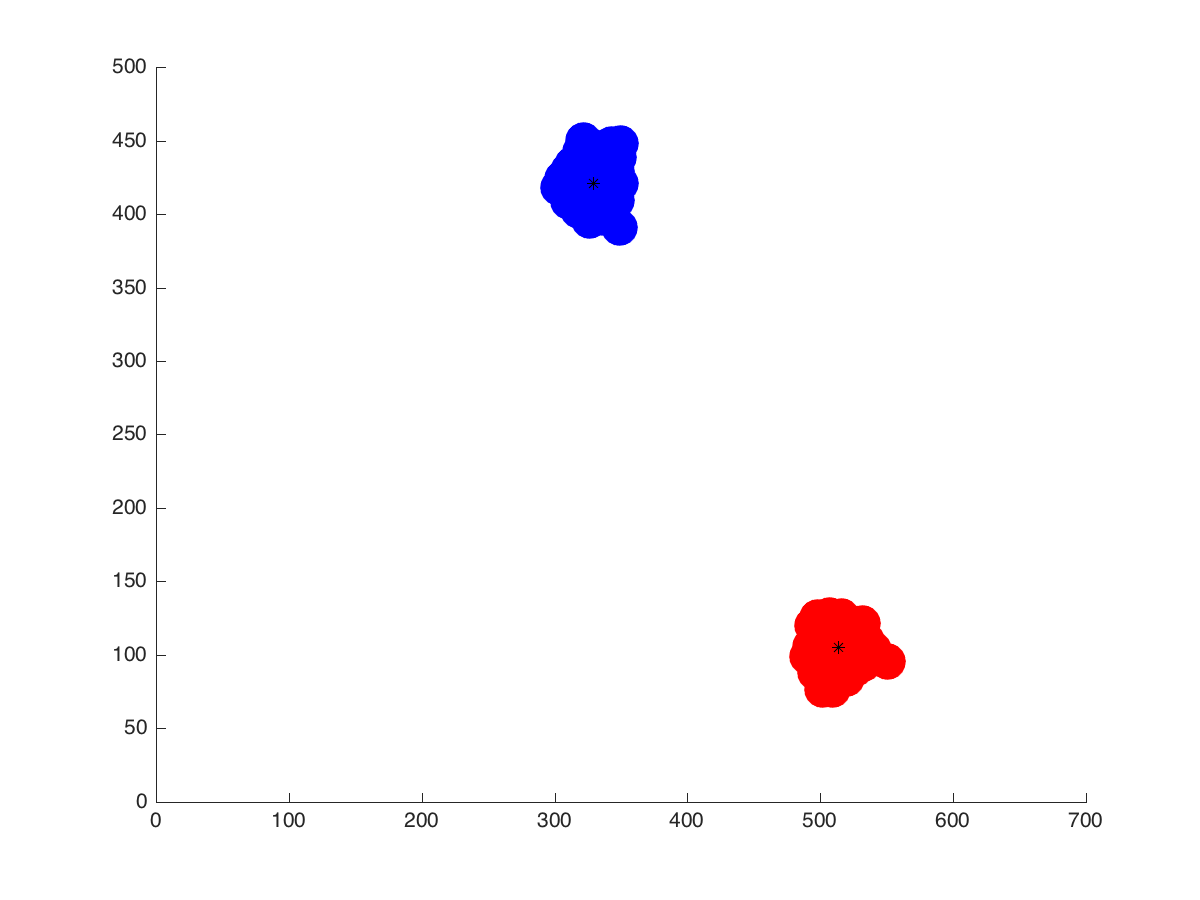
\includegraphics[width=1\textwidth]{figures/Scene.png}
    \captionof{figure}{Scene representation}
    \label{fig:scene}
  \end{minipage}
  \hfill
  \begin{minipage}[b]{0.55\textwidth}
    \centering
    \begin{tabular}{cc}\hline
        \textbf{Reward} & \textbf{Action Condition}\\ \hline
	\\        
        \textcolor{ForestGreen}{+30} & Grasp \textbf{\textcolor{red}{red}} item \\
        \textcolor{ForestGreen}{+10} & Grasp \textbf{\textcolor{blue}{blue}} item \\
        \textcolor{OrangeRed}{-100} & Miss item grasp by 11px \\
        \textcolor{OrangeRed}{-1} & Per item not attempted \\
	\\
        \hline
        \\
        
      \end{tabular}
      \captionof{table}{Rewords for the agent's training}
      \label{table:rewards}
    \end{minipage}

\begin{figure}[h]
	\centering
	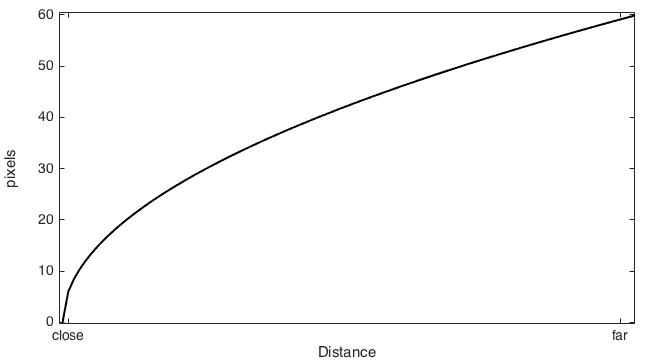
\includegraphics[width=0.7\textwidth]{figures/Noise.png}
	\caption{Function of noisy displacement as distance increases}
	\label{fig:noise}
\end{figure}

The scenario forces a competitive decision between the items to give focus to. 
The world state is represented by the position of the two items, although, due to noisy perception the subject must estimate what those positions are.
As there is time only to accurately observe a single item, subjects must decide which item is more optimal to gain certainty of. 
The scenario therefore constrains subjects to perform in a situation requiring optimal gaze control. 

\section{Representing Uncertainty}
In order to support robust decision making, one must represent the amount of uncertainty present in the world. 
That is, given prior received information, how credible is the posterior belief about an item's position. 
As mentioned previously, nature may employ a form of Bayesian inference for this process.
Following past work on models of gaze control\cite{nunezvarela2013}, our model mimics inference and represents uncertainty through the use of particle filters.

Particle filters are a technique used in robotics to estimate the state of a system given noisy sensory hardware\cite{thrun2005}.
Through it's operation, the filter emulates the effects of Bayesian inference.   
For example, given the current set of information, particles cluster around the approximate location of an observed item.
As new information becomes available, the particles gather tighter around the item's location.
This indicates both a decrease in uncertainty and a better approximation of position. 
The process is best described in figure \ref{fig:uncertainty}, in how uncertainty gradually decreases to eventually represent the likely state of the world. 

\begin{figure}[!h]
	\centering
	\includegraphics[width=0.77\textwidth]{figures/uncertainty.png}
	\caption{Visual information decreasing uncertainty}
	\label{fig:uncertainty}
\end{figure}

We denote the spread of particles for each item to be the agent's belief state. 

\section{Learning From Feedback}
Optimising gaze control requires finding appropriate action policies for an agent to follow.  
For example, at what moment is uncertainty low enough for an item to be safely grasped? 
The answer is situation specific, as it depends on the level of noise present in a system. 
An agent can learn appropriate grasp policies by following methods described in Rashej Rao's decision making under uncertainty \cite{rao2010}.

\begin{figure}[!h]
	\centering
	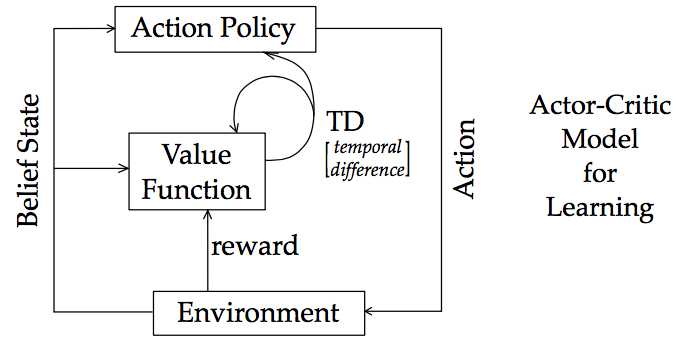
\includegraphics[width=0.9\textwidth]{figures/actorcritic.png}
	\caption{}
	\label{fig:actor-critic}
\end{figure} 

Our agent is trained over 8000 trials using reinforcement learning and an actor critic model (fig. \ref{fig:actor-critic}). 
The model's value function returns the expected reward for the agent's current belief state.
For example, in high uncertainty, the expected reward is low regardless of what actions can be taken.
When uncertainty is low however, the chances of receiving reward are high even if non-optimal decisions are made.  
The mean position of particles in a filter is taken as the estimated item location.
If the particle spread is large, in uncertainty, the item's location is unlikely to be estimated correctly. 

The difference over time steps in a value function is used to train a corresponding action policy.
There are two policies the agent must learn: when to grasp and which item to gaze at.
Therefore, there are two value functions as well. 
The action policy returns the probability with which an agent should execute an action given its current belief state.
For grasping, the policy returns the probability of attempting to grasp an item given its uncertainty spread.
For gazing, the policy returns the probability of focusing at one item or the other given their respective values and level of uncertainty.

\pagebreak
Each pair of value function and action policy are learned using radial basis function(RBF) networks (fig. \ref{fig:rbf}).

\begin{figure}[!h]
	\centering
	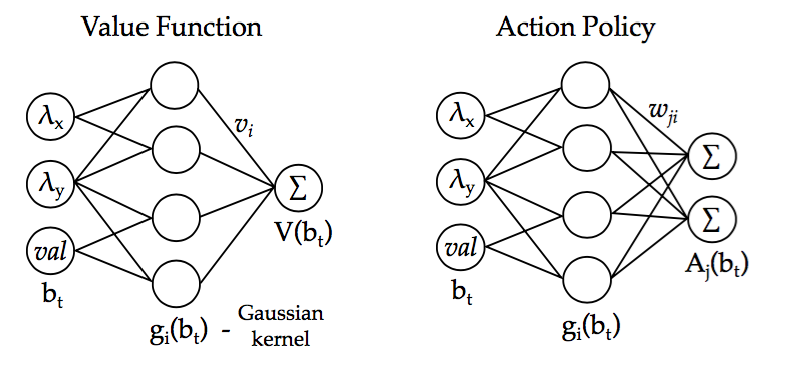
\includegraphics[width=0.8\textwidth]{figures/rbf.png}
	\caption{}
	\label{fig:rbf}
\end{figure} 

The components of the RBF networks are:
\begin{list}{}{}
  \item $\pmb{b_t}$ - is the belief state at time step \emph{t}; represented by an item's particle filter spread (eigenvalues) and the item's reward. 

 \item $\pmb{g_i}$ - is a non-linear Gaussian kernel function ($\sigma=0.25$).
   The kernel centers($\mu$), also known as belief points, act as a receptive field for the belief state.

 \item $\pmb{v_i}$ \& $\pmb{w_i}$ - output layer weights, similar to a feed forward network

 \item $\pmb{V(b_t)}= \Sigma[v_i * g_i(b_t)]$ - value function

 \item $\pmb{A_j(b_t)}= \Sigma[w_{ji} * g_i(b_t)]$ - action value.
   Although network output is the probability $P_{action} = softmax(A_1(b_t),A_2(b_t))$; 
   (where \textbf{softmax} is a normalised exponential function).
\end{list}

Grasp learning requires only a single item's uncertainty and value, whilst gazing requires both. 
This is due to grasping only relying on a single item's uncertainty spread to succeed.
Gazing however brings a competitive decision between the low and high value items.
Gazing therefore requires knowledge of both items for a decision to be made (fig. \ref{fig:inout}). 

\begin{figure}[!h]
	\centering
	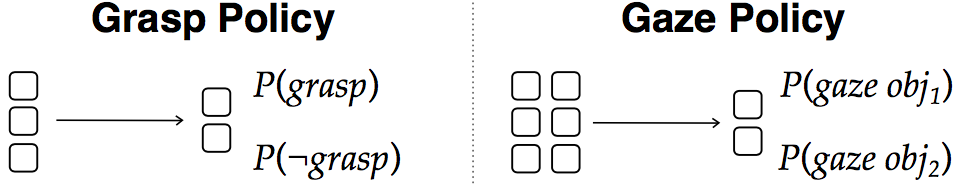
\includegraphics[width=0.8\textwidth]{figures/inputoutput.png}
	\caption{Grasping takes the X-Y coordinate eigenvalues and the value of a single item. Gazing takes both item eigenvalues and reward values.}
	\label{fig:inout}
\end{figure}

Grasp learning is trained in an online fashion using reinforcement learning.
The Gaussian layer of the network is determined prior to training through k-means clustering across a set of randomly generated belief state values.
Our architecture consists of 60 units for the Gaussian layer. 
Reinforcement learning is used to training the output layer weights.
We use the reward values generated by the environment to train these weights. 
At each training step, the weights are updated as follows:

\begin{list}{}{}
  \item \textbf{reward = received from environment}; see table \ref{table:rewards}
  \item $\pmb{TD = reward + V(b_{t+1}) - V(b_t)}$; temporal difference
  \item $\pmb{v_i = v_i + 0.001 * TD * g_i(b_t)}$; value function weights
  \item $\pmb{w_{ji} = w_{ji}+ 0.0005 * TD * g_i(b_t)}$; action policy weights
\end{list}  

Gazeing is trained in a similar manner. 
The Gaussian layer consists of 180 kernel centres that are distributed through k-means clustering. 
However, in training the output layer, the reward is taken as the overall improvement over expected grasping rewards. 
Environment rewards do not directly feed into optimal gaze learning, meaning the model does not exclusively focus on the item rendering highest reward.
Instead, gaze actions depend on an estimated reward value generated by the grasp policy.
More exactly, gaze learning depends on a prediction of the joint improvement of reward over both items.
The improvement stems from a decrease in uncertainty of each item, as new visual information is collected. 

Since the grasping reward increases concomitantly with the probability of executing a grasp action, gaze reward values can be taken as the grasp probabilities instead of actual policy values. 
Changes to environment reward values or to grasp learning rates would not cause further changes in gaze learning as input values are naturally normalised as probabilities.
The update equations for gaze learning are therefore as follows: 
\begin{list}{}{}
  \item $\pmb{reward = \sum_{item}[P_{grasp}(b_{t+1}) -  P_{grasp}(b_t)] }$; 
  \item $\pmb{TD = reward - V(b_t)}$; temporal difference
  \item $\pmb{ v_i = v_i + 0.8 * TD * g_i(b_t)}$; value function weights
  \item $\pmb{w_{ji} = w_{ji}+ 0.4 * TD * g_i(b_t)}$; action policy weights
\end{list}  

\section{Results}
From positive and negative feedback the model was able to learn both grasping and optimised gaze policies.
To establish a baseline for performance, cumulative reward was recorded for a model learning only grasp actions whilst randomly choosing which item to focus on.
Figure \ref{fig:results} shows the effect of optimised gaze compared to random gazing. 
Both procedures show patterns of learning, with low scores at the start of training and high scores at the end.   
Noticeably, optimised gaze performs much better.

\begin{figure}[!h]
	\centering
	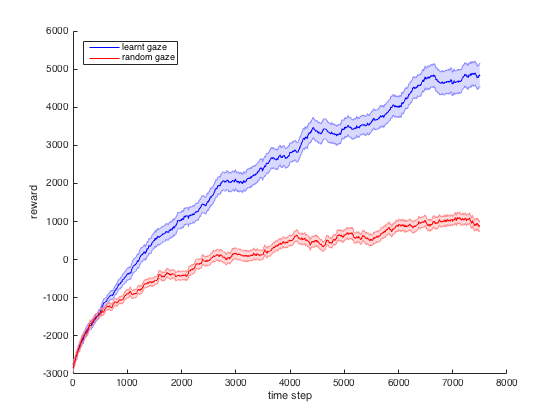
\includegraphics[width=0.9\textwidth]{figures/results.png}
	\caption{Graph shows the actual model performance for the task averaged over 100 trials. The faded blue and red areas indicate the standard error.}
	\label{fig:results}
\end{figure}

Additionally, we explore the scenario where an agent is allowed to make as many visual fixations as needed before having to make grasp decisions. 
The agent is allowed to grasp either object or both, although he may do so when having gained enough certainty about each item's position. 
We incentivise eager grasping by penalising the agent for each time step where it chooses to not grasp.
Figure \ref{fig:resultsTimless} shows optimal gaze to have a marginal impact on overall task performance.
However, when looking at the number of fixations, optimal gaze tends to fixate noticeably fewer times than random gaze (fig. \ref{fig:gazeCount}). 

\begin{figure}[!h]
	\centering
	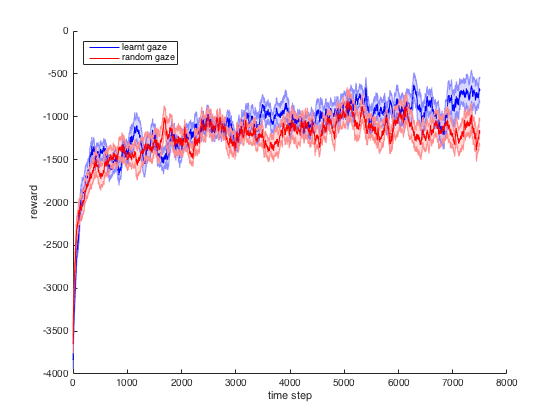
\includegraphics[width=0.9\textwidth]{figures/resultsTimeless.png}
	\caption{Cumulative reward when not limiting the number of ocular fixations.}
	\label{fig:resultsTimless}
\end{figure}


\begin{figure}[!h]
	\centering
	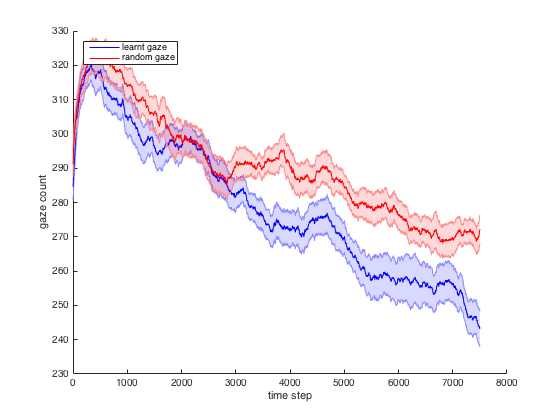
\includegraphics[width=0.9\textwidth]{figures/gazeCount.png}
	\caption{Cumulative number of ocular fixations before a grasp attempt.}
	\label{fig:gazeCount}
\end{figure}

\pagebreak
\printbibliography

\end{document}
